\documentclass[1p]{elsarticle_modified}
%\bibliographystyle{elsarticle-num}

%\usepackage[colorlinks]{hyperref}
%\usepackage{abbrmath_seonhwa} %\Abb, \Ascr, \Acal ,\Abf, \Afrak
\usepackage{amsfonts}
\usepackage{amssymb}
\usepackage{amsmath}
\usepackage{amsthm}
\usepackage{scalefnt}
\usepackage{amsbsy}
\usepackage{kotex}
\usepackage{caption}
\usepackage{subfig}
\usepackage{color}
\usepackage{graphicx}
\usepackage{xcolor} %% white, black, red, green, blue, cyan, magenta, yellow
\usepackage{float}
\usepackage{setspace}
\usepackage{hyperref}

\usepackage{tikz}
\usetikzlibrary{arrows}

\usepackage{multirow}
\usepackage{array} % fixed length table
\usepackage{hhline}

%%%%%%%%%%%%%%%%%%%%%
\makeatletter
\renewcommand*\env@matrix[1][\arraystretch]{%
	\edef\arraystretch{#1}%
	\hskip -\arraycolsep
	\let\@ifnextchar\new@ifnextchar
	\array{*\c@MaxMatrixCols c}}
\makeatother %https://tex.stackexchange.com/questions/14071/how-can-i-increase-the-line-spacing-in-a-matrix
%%%%%%%%%%%%%%%

\usepackage[normalem]{ulem}

\newcommand{\msout}[1]{\ifmmode\text{\sout{\ensuremath{#1}}}\else\sout{#1}\fi}
%SOURCE: \msout is \stkout macro in https://tex.stackexchange.com/questions/20609/strikeout-in-math-mode

\newcommand{\cancel}[1]{
	\ifmmode
	{\color{red}\msout{#1}}
	\else
	{\color{red}\sout{#1}}
	\fi
}

\newcommand{\add}[1]{
	{\color{blue}\uwave{#1}}
}

\newcommand{\replace}[2]{
	\ifmmode
	{\color{red}\msout{#1}}{\color{blue}\uwave{#2}}
	\else
	{\color{red}\sout{#1}}{\color{blue}\uwave{#2}}
	\fi
}

\newcommand{\Sol}{\mathcal{S}} %segment
\newcommand{\D}{D} %diagram
\newcommand{\A}{\mathcal{A}} %arc


%%%%%%%%%%%%%%%%%%%%%%%%%%%%%5 test

\def\sl{\operatorname{\textup{SL}}(2,\Cbb)}
\def\psl{\operatorname{\textup{PSL}}(2,\Cbb)}
\def\quan{\mkern 1mu \triangleright \mkern 1mu}

\theoremstyle{definition}
\newtheorem{thm}{Theorem}[section]
\newtheorem{prop}[thm]{Proposition}
\newtheorem{lem}[thm]{Lemma}
\newtheorem{ques}[thm]{Question}
\newtheorem{cor}[thm]{Corollary}
\newtheorem{defn}[thm]{Definition}
\newtheorem{exam}[thm]{Example}
\newtheorem{rmk}[thm]{Remark}
\newtheorem{alg}[thm]{Algorithm}

\newcommand{\I}{\sqrt{-1}}
\begin{document}

%\begin{frontmatter}
%
%\title{Boundary parabolic representations of knots up to 8 crossings}
%
%%% Group authors per affiliation:
%\author{Yunhi Cho} 
%\address{Department of Mathematics, University of Seoul, Seoul, Korea}
%\ead{yhcho@uos.ac.kr}
%
%
%\author{Seonhwa Kim} %\fnref{s_kim}}
%\address{Center for Geometry and Physics, Institute for Basic Science, Pohang, 37673, Korea}
%\ead{ryeona17@ibs.re.kr}
%
%\author{Hyuk Kim}
%\address{Department of Mathematical Sciences, Seoul National University, Seoul 08826, Korea}
%\ead{hyukkim@snu.ac.kr}
%
%\author{Seokbeom Yoon}
%\address{Department of Mathematical Sciences, Seoul National University, Seoul, 08826,  Korea}
%\ead{sbyoon15@snu.ac.kr}
%
%\begin{abstract}
%We find all boundary parabolic representation of knots up to 8 crossings.
%
%\end{abstract}
%\begin{keyword}
%    \MSC[2010] 57M25 
%\end{keyword}
%
%\end{frontmatter}

%\linenumbers
%\tableofcontents
%
\newcommand\colored[1]{\textcolor{white}{\rule[-0.35ex]{0.8em}{1.4ex}}\kern-0.8em\color{red} #1}%
%\newcommand\colored[1]{\textcolor{white}{ #1}\kern-2.17ex	\textcolor{white}{ #1}\kern-1.81ex	\textcolor{white}{ #1}\kern-2.15ex\color{red}#1	}

{\Large $\underline{12a_{0733}~(K12a_{0733})}$}

\setlength{\tabcolsep}{10pt}
\renewcommand{\arraystretch}{1.6}
\vspace{1cm}\begin{tabular}{m{100pt}>{\centering\arraybackslash}m{274pt}}
\multirow{5}{120pt}{
	\centering
	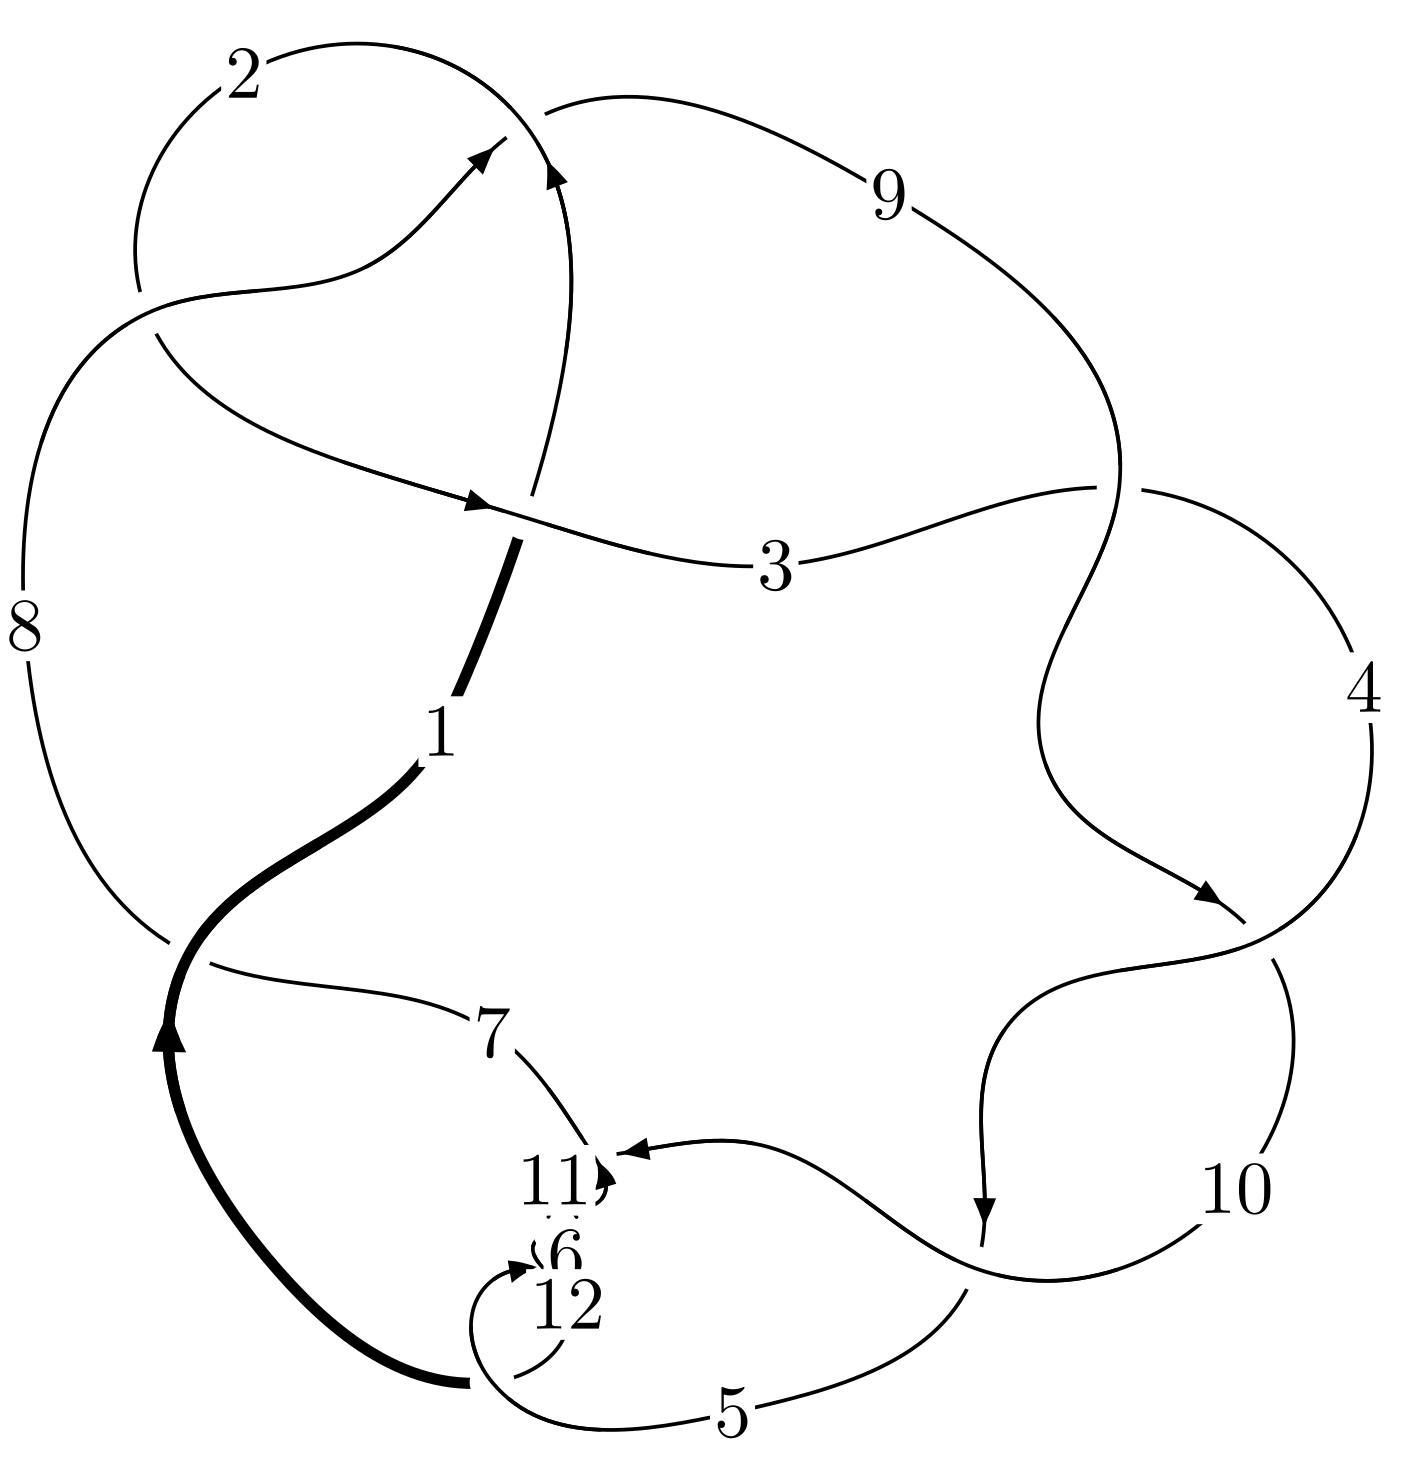
\includegraphics[width=112pt]{../../../GIT/diagram.site/Diagrams/png/1534_12a_0733.png}\\
\ \ \ A knot diagram\footnotemark}&
\allowdisplaybreaks
\textbf{Linearized knot diagam} \\
\cline{2-2}
 &
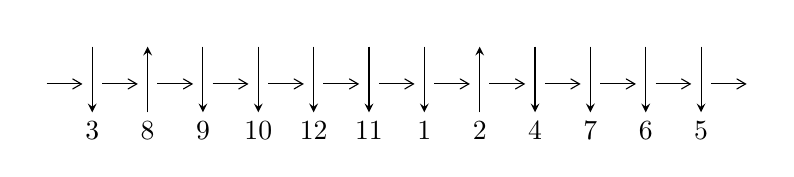
\begin{tikzpicture}[x=20pt, y=17pt]
	% nodes
	\node (C0) at (0, 0) {};
	\node (C1) at (1, 0) {};
	\node (C1U) at (1, +1) {};
	\node (C1D) at (1, -1) {3};

	\node (C2) at (2, 0) {};
	\node (C2U) at (2, +1) {};
	\node (C2D) at (2, -1) {8};

	\node (C3) at (3, 0) {};
	\node (C3U) at (3, +1) {};
	\node (C3D) at (3, -1) {9};

	\node (C4) at (4, 0) {};
	\node (C4U) at (4, +1) {};
	\node (C4D) at (4, -1) {10};

	\node (C5) at (5, 0) {};
	\node (C5U) at (5, +1) {};
	\node (C5D) at (5, -1) {12};

	\node (C6) at (6, 0) {};
	\node (C6U) at (6, +1) {};
	\node (C6D) at (6, -1) {11};

	\node (C7) at (7, 0) {};
	\node (C7U) at (7, +1) {};
	\node (C7D) at (7, -1) {1};

	\node (C8) at (8, 0) {};
	\node (C8U) at (8, +1) {};
	\node (C8D) at (8, -1) {2};

	\node (C9) at (9, 0) {};
	\node (C9U) at (9, +1) {};
	\node (C9D) at (9, -1) {4};

	\node (C10) at (10, 0) {};
	\node (C10U) at (10, +1) {};
	\node (C10D) at (10, -1) {7};

	\node (C11) at (11, 0) {};
	\node (C11U) at (11, +1) {};
	\node (C11D) at (11, -1) {6};

	\node (C12) at (12, 0) {};
	\node (C12U) at (12, +1) {};
	\node (C12D) at (12, -1) {5};
	\node (C13) at (13, 0) {};

	% arrows
	\draw[->,>={angle 60}]
	(C0) edge (C1) (C1) edge (C2) (C2) edge (C3) (C3) edge (C4) (C4) edge (C5) (C5) edge (C6) (C6) edge (C7) (C7) edge (C8) (C8) edge (C9) (C9) edge (C10) (C10) edge (C11) (C11) edge (C12) (C12) edge (C13) ;	\draw[->,>=stealth]
	(C1U) edge (C1D) (C2D) edge (C2U) (C3U) edge (C3D) (C4U) edge (C4D) (C5U) edge (C5D) (C6U) edge (C6D) (C7U) edge (C7D) (C8D) edge (C8U) (C9U) edge (C9D) (C10U) edge (C10D) (C11U) edge (C11D) (C12U) edge (C12D) ;
	\end{tikzpicture} \\
\hhline{~~} \\& 
\textbf{Solving Sequence} \\ \cline{2-2} 
 &
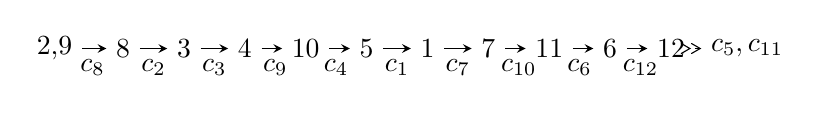
\begin{tikzpicture}[x=22pt, y=7pt]
	% node
	\node (A0) at (-1/8, 0) {2,9};
	\node (A1) at (1, 0) {8};
	\node (A2) at (2, 0) {3};
	\node (A3) at (3, 0) {4};
	\node (A4) at (4, 0) {10};
	\node (A5) at (5, 0) {5};
	\node (A6) at (6, 0) {1};
	\node (A7) at (7, 0) {7};
	\node (A8) at (8, 0) {11};
	\node (A9) at (9, 0) {6};
	\node (A10) at (10, 0) {12};
	\node (C1) at (1/2, -1) {$c_{8}$};
	\node (C2) at (3/2, -1) {$c_{2}$};
	\node (C3) at (5/2, -1) {$c_{3}$};
	\node (C4) at (7/2, -1) {$c_{9}$};
	\node (C5) at (9/2, -1) {$c_{4}$};
	\node (C6) at (11/2, -1) {$c_{1}$};
	\node (C7) at (13/2, -1) {$c_{7}$};
	\node (C8) at (15/2, -1) {$c_{10}$};
	\node (C9) at (17/2, -1) {$c_{6}$};
	\node (C10) at (19/2, -1) {$c_{12}$};
	\node (A11) at (45/4, 0) {$c_{5},c_{11}$};

	% edge
	\draw[->,>=stealth]	
	(A0) edge (A1) (A1) edge (A2) (A2) edge (A3) (A3) edge (A4) (A4) edge (A5) (A5) edge (A6) (A6) edge (A7) (A7) edge (A8) (A8) edge (A9) (A9) edge (A10) ;
	\draw[->>,>={angle 60}]	
	(A10) edge (A11);
\end{tikzpicture} \\ 

\end{tabular} \\

\footnotetext{
The image of knot diagram is generated by the software ``\textbf{Draw programme}" developed by Andrew Bartholomew(\url{http://www.layer8.co.uk/maths/draw/index.htm\#Running-draw}), where we modified some parts for our purpose(\url{https://github.com/CATsTAILs/LinksPainter}).
}\phantom \\ \newline 
\centering \textbf{Ideals for irreducible components\footnotemark of $X_{\text{par}}$} 
 
\begin{align*}
I^u_{1}&=\langle 
u^{36}- u^{35}+\cdots+u^2-1\rangle \\
\\
\end{align*}
\raggedright * 1 irreducible components of $\dim_{\mathbb{C}}=0$, with total 36 representations.\\
\footnotetext{All coefficients of polynomials are rational numbers. But the coefficients are sometimes approximated in decimal forms when there is not enough margin.}
\newpage
\renewcommand{\arraystretch}{1}
\centering \section*{I. $I^u_{1}= \langle u^{36}- u^{35}+\cdots+u^2-1 \rangle$}
\flushleft \textbf{(i) Arc colorings}\\
\begin{tabular}{m{7pt} m{180pt} m{7pt} m{180pt} }
\flushright $a_{2}=$&$\begin{pmatrix}0\\u\end{pmatrix}$ \\
\flushright $a_{9}=$&$\begin{pmatrix}1\\0\end{pmatrix}$ \\
\flushright $a_{8}=$&$\begin{pmatrix}1\\u^2\end{pmatrix}$ \\
\flushright $a_{3}=$&$\begin{pmatrix}u\\u^3+u\end{pmatrix}$ \\
\flushright $a_{4}=$&$\begin{pmatrix}- u^3\\u^3+u\end{pmatrix}$ \\
\flushright $a_{10}=$&$\begin{pmatrix}- u^6- u^4+1\\u^6+2 u^4+u^2\end{pmatrix}$ \\
\flushright $a_{5}=$&$\begin{pmatrix}u^9+2 u^7+u^5-2 u^3- u\\- u^9-3 u^7-3 u^5+u\end{pmatrix}$ \\
\flushright $a_{1}=$&$\begin{pmatrix}u^3\\u^5+u^3+u\end{pmatrix}$ \\
\flushright $a_{7}=$&$\begin{pmatrix}- u^6- u^4+1\\- u^8-2 u^6-2 u^4\end{pmatrix}$ \\
\flushright $a_{11}=$&$\begin{pmatrix}- u^{20}-5 u^{18}-11 u^{16}-10 u^{14}+2 u^{12}+13 u^{10}+9 u^8-2 u^6-5 u^4- u^2+1\\- u^{22}-6 u^{20}-17 u^{18}-26 u^{16}-20 u^{14}+13 u^{10}+10 u^8+3 u^6+2 u^4+u^2\end{pmatrix}$ \\
\flushright $a_{6}=$&$\begin{pmatrix}- u^{34}-9 u^{32}+\cdots- u^2+1\\- u^{35}+u^{34}+\cdots+u^2-1\end{pmatrix}$ \\
\flushright $a_{12}=$&$\begin{pmatrix}u^{23}+6 u^{21}+\cdots+6 u^5+2 u^3\\- u^{23}-7 u^{21}+\cdots-3 u^5+u\end{pmatrix}$\\&\end{tabular}
\flushleft \textbf{(ii) Obstruction class $= -1$}\\~\\
\flushleft \textbf{(iii) Cusp Shapes $= 4 u^{35}-4 u^{34}+40 u^{33}-36 u^{32}+188 u^{31}-156 u^{30}+524 u^{29}-408 u^{28}+908 u^{27}-688 u^{26}+880 u^{25}-720 u^{24}+124 u^{23}-340 u^{22}-868 u^{21}+236 u^{20}-1120 u^{19}+600 u^{18}-444 u^{17}+592 u^{16}+280 u^{15}+332 u^{14}+360 u^{13}+20 u^{12}+84 u^{11}-172 u^{10}-60 u^9-156 u^8-24 u^7-52 u^6+16 u^5+4 u^4+20 u^3-10$}\\~\\
\newpage\renewcommand{\arraystretch}{1}
\flushleft \textbf{(iv) u-Polynomials at the component}\newline \\
\begin{tabular}{m{50pt}|m{274pt}}
Crossings & \hspace{64pt}u-Polynomials at each crossing \\
\hline $$\begin{aligned}c_{1}\end{aligned}$$&$\begin{aligned}
&u^{36}+21 u^{35}+\cdots-2 u+1
\end{aligned}$\\
\hline $$\begin{aligned}c_{2},c_{8}\end{aligned}$$&$\begin{aligned}
&u^{36}- u^{35}+\cdots+u^2-1
\end{aligned}$\\
\hline $$\begin{aligned}c_{3},c_{4},c_{7}\\c_{9}\end{aligned}$$&$\begin{aligned}
&u^{36}+u^{35}+\cdots-6 u-5
\end{aligned}$\\
\hline $$\begin{aligned}c_{5},c_{6},c_{10}\\c_{11},c_{12}\end{aligned}$$&$\begin{aligned}
&u^{36}+u^{35}+\cdots-4 u-1
\end{aligned}$\\
\hline
\end{tabular}\\~\\
\newpage\renewcommand{\arraystretch}{1}
\flushleft \textbf{(v) Riley Polynomials at the component}\newline \\
\begin{tabular}{m{50pt}|m{274pt}}
Crossings & \hspace{64pt}Riley Polynomials at each crossing \\
\hline $$\begin{aligned}c_{1}\end{aligned}$$&$\begin{aligned}
&y^{36}-11 y^{35}+\cdots-30 y+1
\end{aligned}$\\
\hline $$\begin{aligned}c_{2},c_{8}\end{aligned}$$&$\begin{aligned}
&y^{36}+21 y^{35}+\cdots-2 y+1
\end{aligned}$\\
\hline $$\begin{aligned}c_{3},c_{4},c_{7}\\c_{9}\end{aligned}$$&$\begin{aligned}
&y^{36}-43 y^{35}+\cdots-166 y+25
\end{aligned}$\\
\hline $$\begin{aligned}c_{5},c_{6},c_{10}\\c_{11},c_{12}\end{aligned}$$&$\begin{aligned}
&y^{36}+45 y^{35}+\cdots-2 y+1
\end{aligned}$\\
\hline
\end{tabular}\\~\\
\newpage\flushleft \textbf{(vi) Complex Volumes and Cusp Shapes}
$$\begin{array}{c|c|c}  
\text{Solutions to }I^u_{1}& \I (\text{vol} + \sqrt{-1}CS) & \text{Cusp shape}\\
 \hline 
\begin{aligned}
u &= \phantom{-}0.282875 + 1.062700 I\end{aligned}
 & -1.68586 + 0.53085 I & -10.75192 + 0.82754 I \\ \hline\begin{aligned}
u &= \phantom{-}0.282875 - 1.062700 I\end{aligned}
 & -1.68586 - 0.53085 I & -10.75192 - 0.82754 I \\ \hline\begin{aligned}
u &= \phantom{-}0.891515 + 0.048885 I\end{aligned}
 & \phantom{-}2.90046 - 5.74969 I & -5.68594 + 2.68814 I \\ \hline\begin{aligned}
u &= \phantom{-}0.891515 - 0.048885 I\end{aligned}
 & \phantom{-}2.90046 + 5.74969 I & -5.68594 - 2.68814 I \\ \hline\begin{aligned}
u &= \phantom{-}0.890163\phantom{ +0.000000I}\end{aligned}
 & -8.32989\phantom{ +0.000000I} & -11.7240\phantom{ +0.000000I} \\ \hline\begin{aligned}
u &= -0.888293 + 0.024901 I\end{aligned}
 & -5.76957 + 3.65801 I & -7.50646 - 3.88825 I \\ \hline\begin{aligned}
u &= -0.888293 - 0.024901 I\end{aligned}
 & -5.76957 - 3.65801 I & -7.50646 + 3.88825 I \\ \hline\begin{aligned}
u &= \phantom{-}0.498093 + 0.734304 I\end{aligned}
 & \phantom{-}12.00850 + 2.05861 I & -1.12178 - 3.75231 I \\ \hline\begin{aligned}
u &= \phantom{-}0.498093 - 0.734304 I\end{aligned}
 & \phantom{-}12.00850 - 2.05861 I & -1.12178 + 3.75231 I \\ \hline\begin{aligned}
u &= -0.375034 + 1.064500 I\end{aligned}
 & -3.45066 - 3.25878 I & -14.9165 + 5.6693 I \\ \hline\begin{aligned}
u &= -0.375034 - 1.064500 I\end{aligned}
 & -3.45066 + 3.25878 I & -14.9165 - 5.6693 I \\ \hline\begin{aligned}
u &= -0.210685 + 1.118540 I\end{aligned}
 & \phantom{-}6.42157 + 0.49356 I & -9.63907 + 0.32963 I \\ \hline\begin{aligned}
u &= -0.210685 - 1.118540 I\end{aligned}
 & \phantom{-}6.42157 - 0.49356 I & -9.63907 - 0.32963 I \\ \hline\begin{aligned}
u &= \phantom{-}0.444121 + 1.051070 I\end{aligned}
 & -0.51949 + 5.89850 I & -7.49197 - 8.58873 I \\ \hline\begin{aligned}
u &= \phantom{-}0.444121 - 1.051070 I\end{aligned}
 & -0.51949 - 5.89850 I & -7.49197 + 8.58873 I \\ \hline\begin{aligned}
u &= -0.490379 + 1.047610 I\end{aligned}
 & \phantom{-}8.45002 - 7.20201 I & -5.83680 + 6.79259 I \\ \hline\begin{aligned}
u &= -0.490379 - 1.047610 I\end{aligned}
 & \phantom{-}8.45002 + 7.20201 I & -5.83680 - 6.79259 I \\ \hline\begin{aligned}
u &= -0.405042 + 0.735070 I\end{aligned}
 & \phantom{-}2.86862 - 1.80232 I & -0.91103 + 4.87236 I \\ \hline\begin{aligned}
u &= -0.405042 - 0.735070 I\end{aligned}
 & \phantom{-}2.86862 + 1.80232 I & -0.91103 - 4.87236 I \\ \hline\begin{aligned}
u &= \phantom{-}0.149662 + 0.790037 I\end{aligned}
 & -0.605604 + 0.932135 I & -9.94128 - 6.89796 I \\ \hline\begin{aligned}
u &= \phantom{-}0.149662 - 0.790037 I\end{aligned}
 & -0.605604 - 0.932135 I & -9.94128 + 6.89796 I \\ \hline\begin{aligned}
u &= -0.622331 + 0.303894 I\end{aligned}
 & \phantom{-}10.53390 + 2.88470 I & -2.43200 - 2.46197 I \\ \hline\begin{aligned}
u &= -0.622331 - 0.303894 I\end{aligned}
 & \phantom{-}10.53390 - 2.88470 I & -2.43200 + 2.46197 I \\ \hline\begin{aligned}
u &= \phantom{-}0.439815 + 1.266880 I\end{aligned}
 & -1.13178 - 1.06458 I & -9.26896 - 0.31777 I \\ \hline\begin{aligned}
u &= \phantom{-}0.439815 - 1.266880 I\end{aligned}
 & -1.13178 + 1.06458 I & -9.26896 + 0.31777 I \\ \hline\begin{aligned}
u &= -0.454338 + 1.261880 I\end{aligned}
 & -9.69160 - 1.09254 I & -10.99035 - 0.80742 I \\ \hline\begin{aligned}
u &= -0.454338 - 1.261880 I\end{aligned}
 & -9.69160 + 1.09254 I & -10.99035 + 0.80742 I \\ \hline\begin{aligned}
u &= -0.481098 + 1.254150 I\end{aligned}
 & -9.49472 - 8.55149 I & -10.56405 + 6.84602 I \\ \hline\begin{aligned}
u &= -0.481098 - 1.254150 I\end{aligned}
 & -9.49472 + 8.55149 I & -10.56405 - 6.84602 I \\ \hline\begin{aligned}
u &= \phantom{-}0.468539 + 1.259380 I\end{aligned}
 & -12.15810 + 4.83267 I & -14.8489 - 3.1819 I\\
 \hline 
 \end{array}$$\newpage$$\begin{array}{c|c|c}  
\text{Solutions to }I^u_{1}& \I (\text{vol} + \sqrt{-1}CS) & \text{Cusp shape}\\
 \hline 
\begin{aligned}
u &= \phantom{-}0.468539 - 1.259380 I\end{aligned}
 & -12.15810 - 4.83267 I & -14.8489 + 3.1819 I \\ \hline\begin{aligned}
u &= \phantom{-}0.493269 + 1.250710 I\end{aligned}
 & -0.73827 + 10.71510 I & -8.69637 - 5.67492 I \\ \hline\begin{aligned}
u &= \phantom{-}0.493269 - 1.250710 I\end{aligned}
 & -0.73827 - 10.71510 I & -8.69637 + 5.67492 I \\ \hline\begin{aligned}
u &= \phantom{-}0.539657 + 0.237187 I\end{aligned}
 & \phantom{-}1.69494 - 1.97215 I & -3.23018 + 4.60396 I \\ \hline\begin{aligned}
u &= \phantom{-}0.539657 - 0.237187 I\end{aligned}
 & \phantom{-}1.69494 + 1.97215 I & -3.23018 - 4.60396 I \\ \hline\begin{aligned}
u &= -0.450859\phantom{ +0.000000I}\end{aligned}
 & -0.804226\phantom{ +0.000000I} & -12.6090\phantom{ +0.000000I}\\
 \hline 
 \end{array}$$\newpage
\newpage\renewcommand{\arraystretch}{1}
\centering \section*{ II. u-Polynomials}
\begin{tabular}{m{50pt}|m{274pt}}
Crossings & \hspace{64pt}u-Polynomials at each crossing \\
\hline $$\begin{aligned}c_{1}\end{aligned}$$&$\begin{aligned}
&u^{36}+21 u^{35}+\cdots-2 u+1
\end{aligned}$\\
\hline $$\begin{aligned}c_{2},c_{8}\end{aligned}$$&$\begin{aligned}
&u^{36}- u^{35}+\cdots+u^2-1
\end{aligned}$\\
\hline $$\begin{aligned}c_{3},c_{4},c_{7}\\c_{9}\end{aligned}$$&$\begin{aligned}
&u^{36}+u^{35}+\cdots-6 u-5
\end{aligned}$\\
\hline $$\begin{aligned}c_{5},c_{6},c_{10}\\c_{11},c_{12}\end{aligned}$$&$\begin{aligned}
&u^{36}+u^{35}+\cdots-4 u-1
\end{aligned}$\\
\hline
\end{tabular}\newpage\renewcommand{\arraystretch}{1}
\centering \section*{ III. Riley Polynomials}
\begin{tabular}{m{50pt}|m{274pt}}
Crossings & \hspace{64pt}Riley Polynomials at each crossing \\
\hline $$\begin{aligned}c_{1}\end{aligned}$$&$\begin{aligned}
&y^{36}-11 y^{35}+\cdots-30 y+1
\end{aligned}$\\
\hline $$\begin{aligned}c_{2},c_{8}\end{aligned}$$&$\begin{aligned}
&y^{36}+21 y^{35}+\cdots-2 y+1
\end{aligned}$\\
\hline $$\begin{aligned}c_{3},c_{4},c_{7}\\c_{9}\end{aligned}$$&$\begin{aligned}
&y^{36}-43 y^{35}+\cdots-166 y+25
\end{aligned}$\\
\hline $$\begin{aligned}c_{5},c_{6},c_{10}\\c_{11},c_{12}\end{aligned}$$&$\begin{aligned}
&y^{36}+45 y^{35}+\cdots-2 y+1
\end{aligned}$\\
\hline
\end{tabular}
\vskip 2pc
\end{document}